%
\includepdf[pages=-]{PALOMARES.pdf}
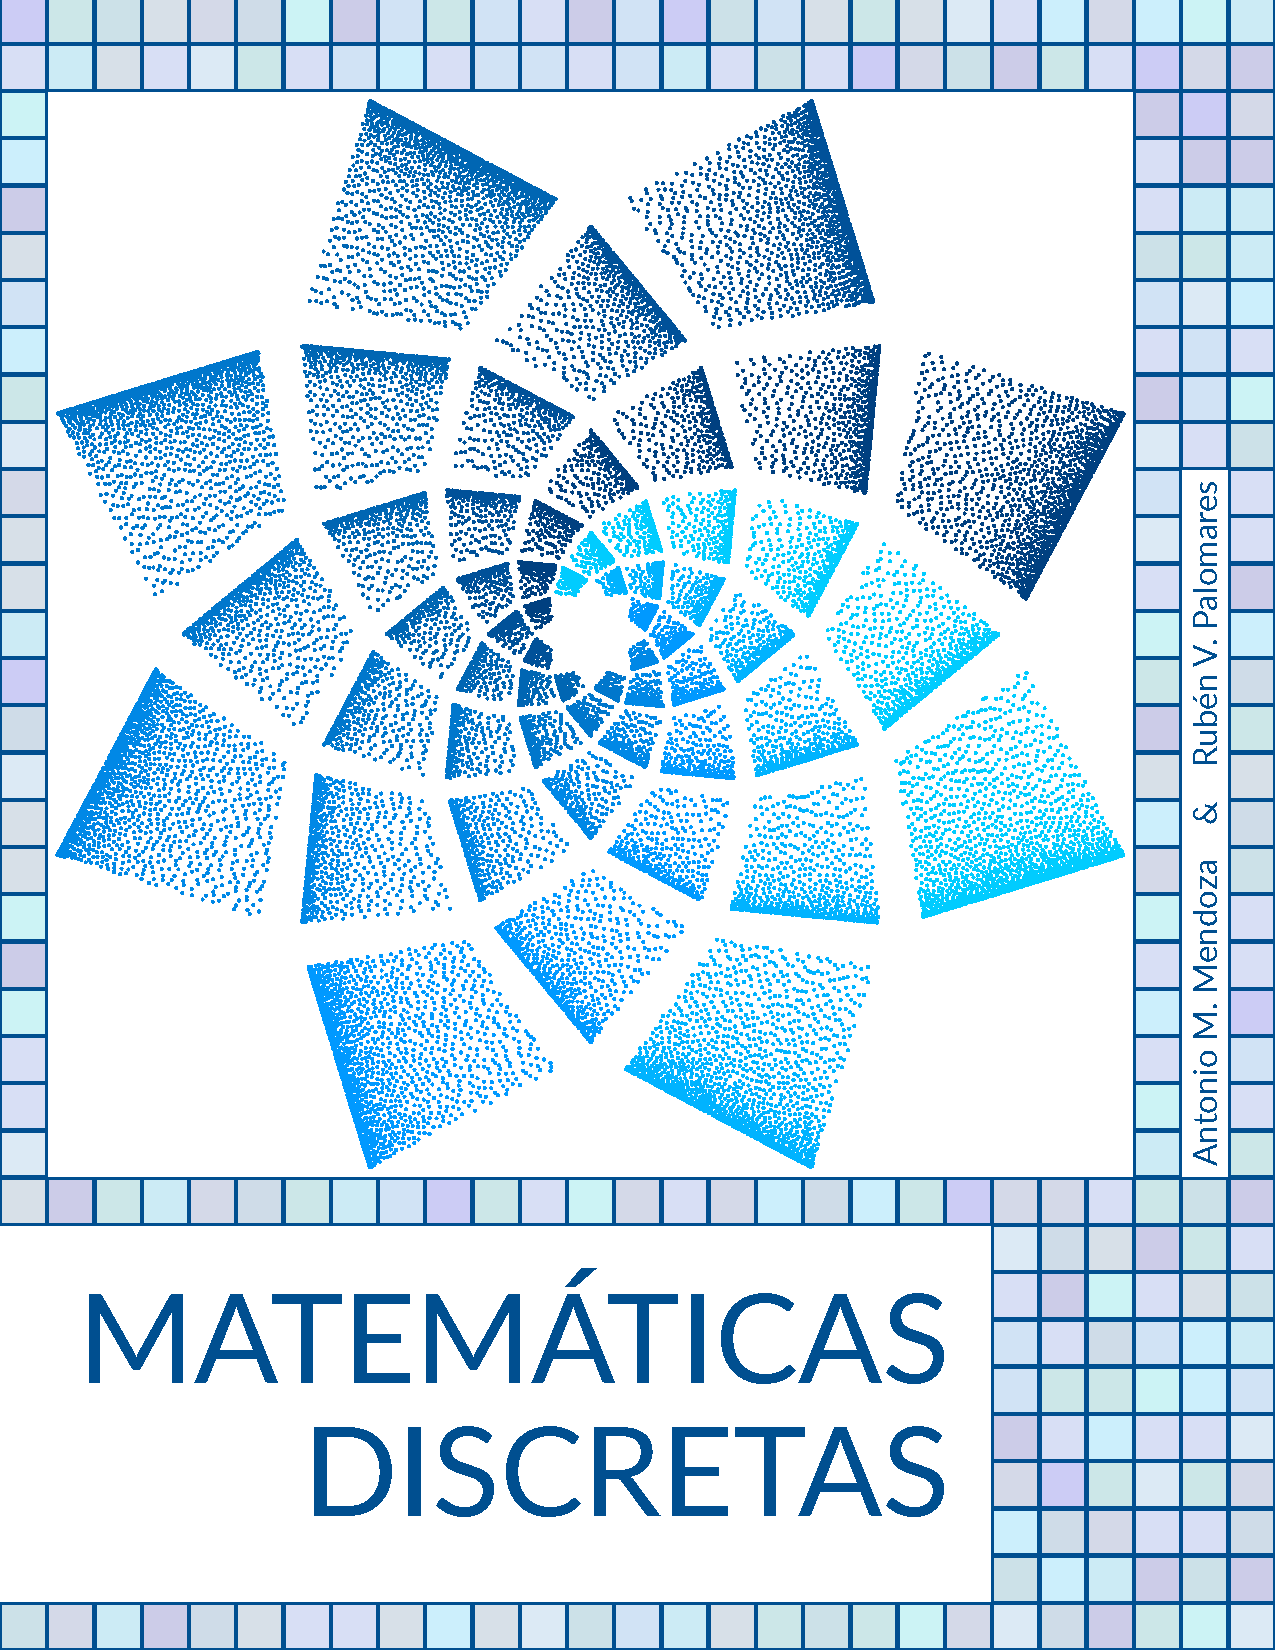
\includepdf[pages=-]{Portada_de_colores.pdf}

\newpage 

\begin{tikzpicture}[remember picture,overlay]%
      \coordinate (A) at ($(current page.north)!.4!(current page.north east)$);
      \coordinate (B) at (current page.east);
      \coordinate (C) at (current page.north east);

      \filldraw[jblueleft] (A) -- (B) -- (C) -- cycle;
\end{tikzpicture}

\,
\vspace{3cm}
\begin{center}
\scalebox{3}{\textbf{\color{jblueleft}MATEMÁTICAS DISCRETAS}}\\
\,
\,\\
\scalebox{2}{\textbf{\color{jblueleft}Una introducción con aplicaciones}}\\
\,\\
\,\\
\scalebox{1.3}{\textbf{\color{jblueleft} Rubén Ramón Vargas Palomares}}\\
\,\\
Profesor de matemáticas de la ESFM\\
\vspace{2cm}
\begin{center}
      \begin{tikzpicture}
            \node at (current page.center) {
\includegraphics[width=0.5\textwidth]{Images/IPNAZUL.pdf}}; % Logo de institución
      \end{tikzpicture}
\end{center}
\vfill
México, 2023
\end{center}

\newpage
\,